\chapter{Appendix 1}\label{app1}
Figure B.1 and B.2 show noise removal working in two contrasting ways 

\begin{figure}[H]
    \centering
    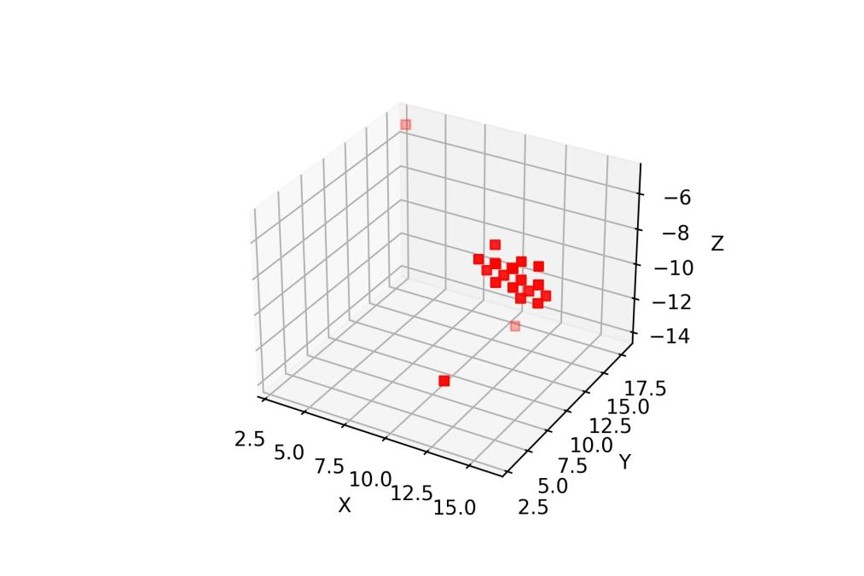
\includegraphics[width=380px, keepaspectratio=true]{appendix1.jpg}
    \caption{Correct noise removal behaviour.}
    \label{fig:my_label}
\end{figure}

\begin{figure}[H]
    \centering
    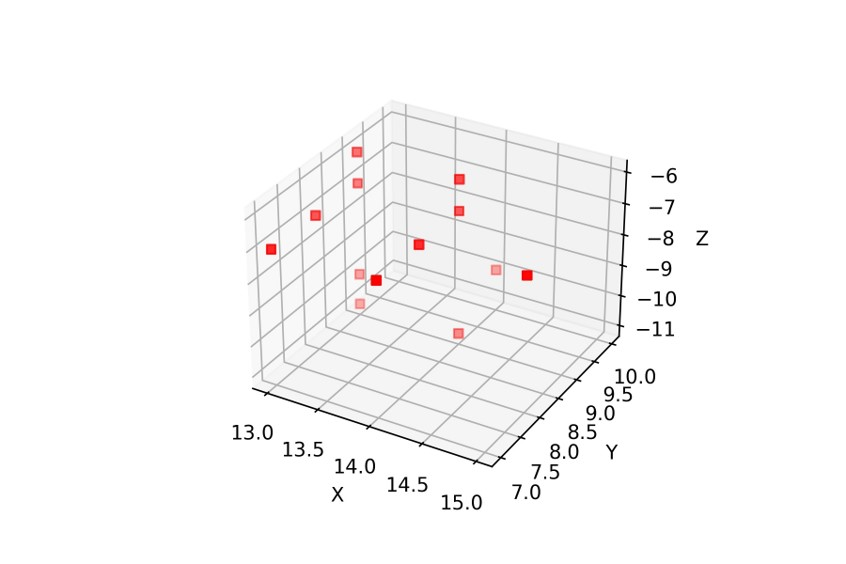
\includegraphics[width=380px, keepaspectratio=true]{appendix2.jpg}
    \caption{Incorrect noise removal behaviour.}
    \label{fig:my_label}
\end{figure}

These next sequence of images show a fall sample frame by frame and display the point clouds corresponding. It can be shown that the target is being lost inconsistenly, polluting the falling sample with noise data. 

\begin{figure}[H]
    \centering
    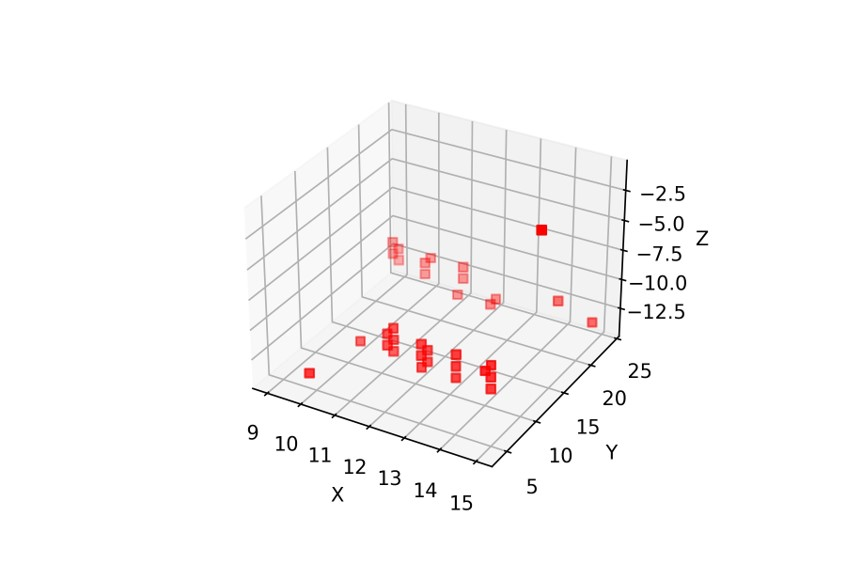
\includegraphics[width=380px, keepaspectratio=true]{appendix3.jpg}
    \caption{Fall frame 1 normal.}
    \label{fig:my_label}
\end{figure}

\begin{figure}[H]
    \centering
    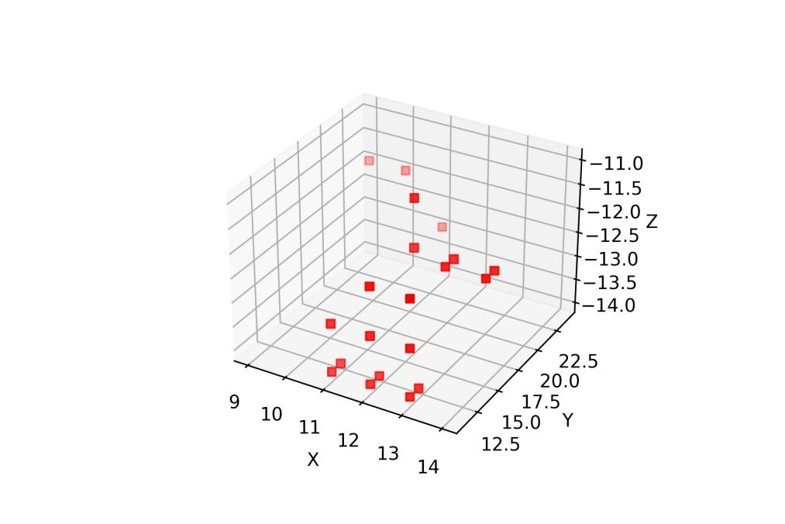
\includegraphics[width=380px, keepaspectratio=true]{appendix4.jpg}
    \caption{Fall frame 2 wrong.}
    \label{fig:my_label}
\end{figure}

\begin{figure}[H]
    \centering
    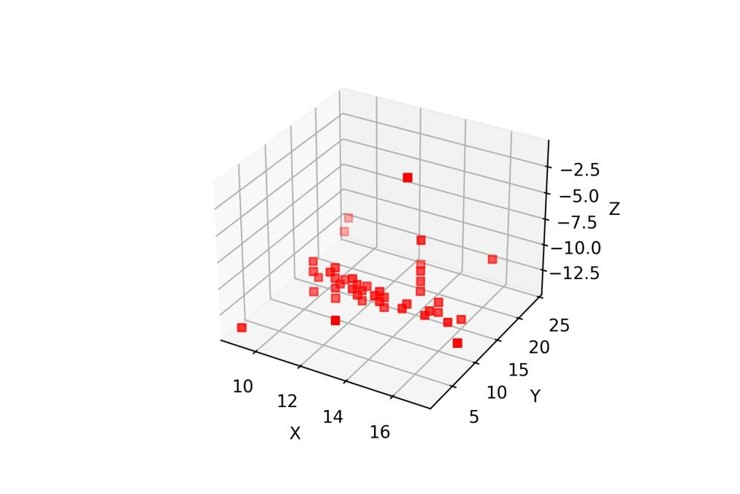
\includegraphics[width=380px, keepaspectratio=true]{appendix5.jpg}
    \caption{Fall frame 3 normal.}
    \label{fig:my_label}
\end{figure}

\begin{figure}[H]
    \centering
    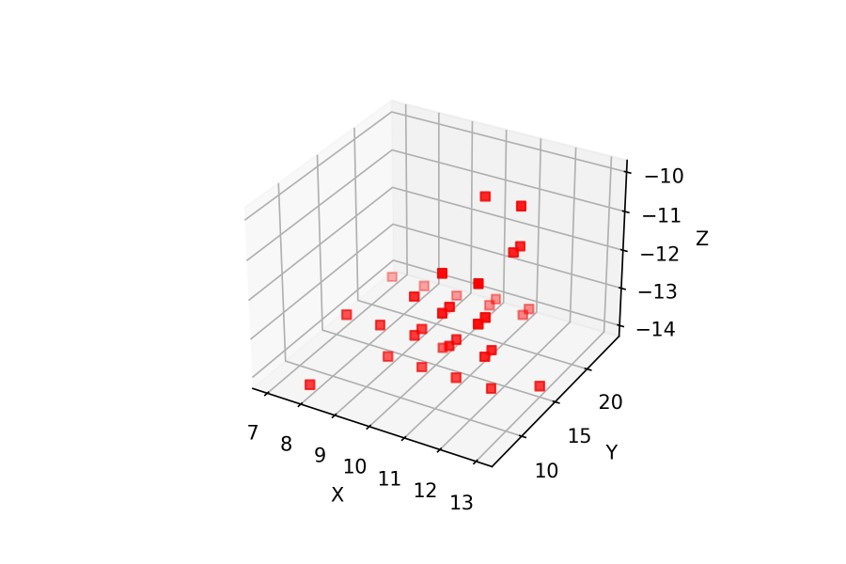
\includegraphics[width=380px, keepaspectratio=true]{appendix6.jpg}
    \caption{Fall frame 4 wrong.}
    \label{fig:my_label}
\end{figure}

\begin{figure}[H]
    \centering
    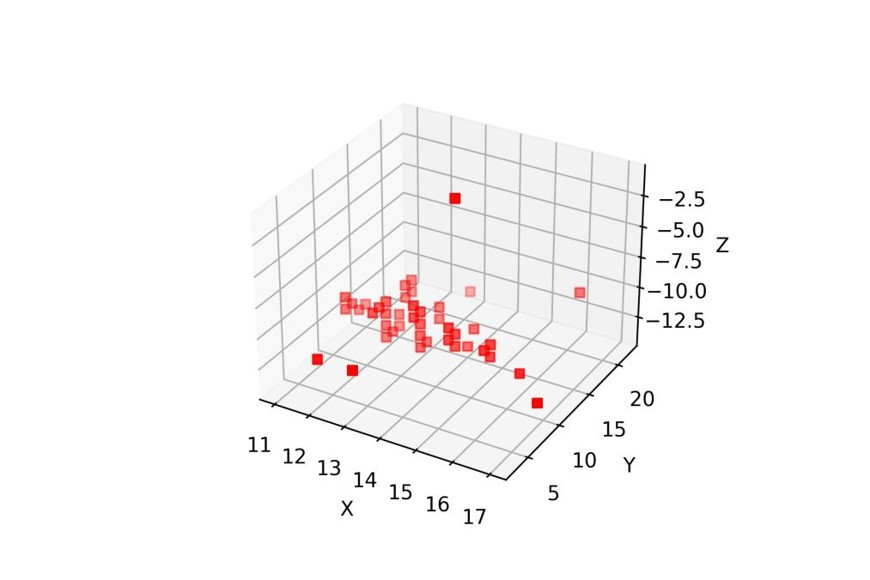
\includegraphics[width=380px, keepaspectratio=true]{appendix7.jpg}
    \caption{Fall frame 5 normal.}
    \label{fig:my_label}
\end{figure}

\begin{figure}[H]
    \centering
    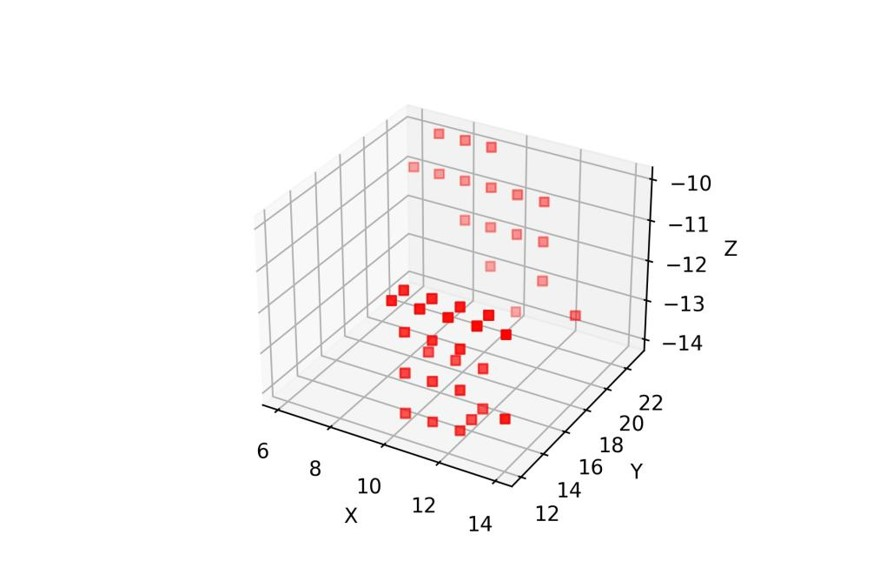
\includegraphics[width=380px, keepaspectratio=true]{appendix8.jpg}
    \caption{Fall frame 6 wrong.}
    \label{fig:my_label}
\end{figure}